% Chapter 4

\chapter{系统测试与结果分析}
\section{无人机系统测试}
\subsection{目标检测测试}
本项目使用基准标记作为搜索目标,图~\ref{fig:4-1}$\sim$~\ref{fig:4-3}为摄像头拍摄的三种基准标记图像的检测结果。可以看到,对于AprilTag,不同型号的标记都可以被正确检测到,但是型号为4×4的标记存在误检现象;对于ChromaTag (只有4×4一种型号),同样可以被正确检测到,但也存在误检现象;对于ArUco标记,不同型号的标记均可以被正确检测出来,但型号为4×4的标记也存在误检现象。然而通过实验发现,误检给出的ID均为17,该ID对应的ArUco标记如图~\ref{fig:4-4}所示,可以看到图案过于简单,因此容易引起误检,而检测算法并非导致误检的主要原因。

通过比较可以发现基准标记的型号越复杂,检测的准确率越高,并且在三种基准标记中,ArUco标记检测的准确率最高。

\begin{figure}[htb]
	\begin{minipage}[t]{0.33\linewidth}
		\centering
		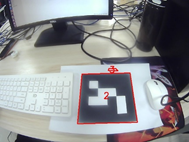
\includegraphics[width=\columnwidth]{figures/4-1a.png} 
		\subcaption{4×4} 
		\label{fig:4-1a} 
	\end{minipage}
	\begin{minipage}[t]{0.33\linewidth} 
		\centering
		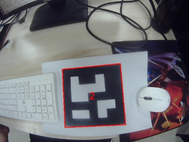
\includegraphics[width=\columnwidth]{figures/4-1b.png} 
		\subcaption{5×5} 
		\label{fig:4-1b} 
	\end{minipage}
	\begin{minipage}[t]{0.33\linewidth} 
		\centering
		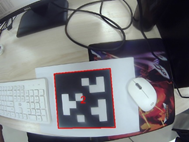
\includegraphics[width=\columnwidth]{figures/4-1c.png} 
		\subcaption{6×6} 
		\label{fig:4-1c} 
	\end{minipage}
	\caption{AprilTag检测结果}
	\label{fig:4-1}
\end{figure}

\begin{figure}[htb]
	\centering
	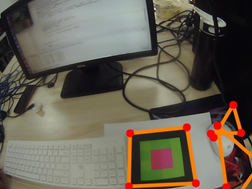
\includegraphics[width=0.4\linewidth]{figures/4-2.png}
	\caption{ChromaTag检测结果}
	\label{fig:4-2}
\end{figure}

\clearpage
\begin{figure}[htb]
	\begin{minipage}[t]{0.33\linewidth}
		\centering
		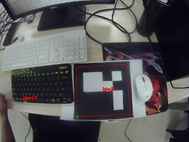
\includegraphics[width=\columnwidth]{figures/4-3a.png} 
		\subcaption{4×4} 
		\label{fig:4-3a} 
	\end{minipage}
	\begin{minipage}[t]{0.33\linewidth} 
		\centering
		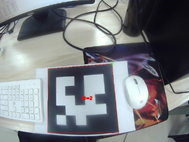
\includegraphics[width=\columnwidth]{figures/4-3b.png} 
		\subcaption{5×5} 
		\label{fig:4-3b} 
	\end{minipage}
	\begin{minipage}[t]{0.33\linewidth} 
		\centering
		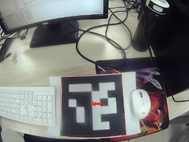
\includegraphics[width=\columnwidth]{figures/4-3c.png} 
		\subcaption{6×6} 
		\label{fig:4-3c} 
	\end{minipage}
	\caption{ArUco标记检测结果}
	\label{fig:4-3}
\end{figure}

\begin{figure}[htb]
	\centering
	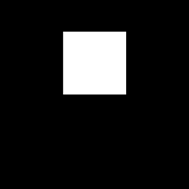
\includegraphics[width=0.33\linewidth]{figures/4-4.png}
	\caption{ID为17的4×4 ArUco标记}
	\label{fig:4-4}
\end{figure}

表~\ref{tab:4-1}为三种基准标记检测的耗时情况测试结果,测试平台为台式电脑,处理器型号为Intel i5-4570,主频为3.2GHz,测试的基准标记数量为0或1。

\begin{table}[htb]
	\centering
	\caption{基准标记检测的耗时情况测试结果}
	\label{tab:4-1}
	\begin{tabular}{ccc}
		\toprule
		基准标记 & 型号  & 平均耗时(ms) \\
		\toprule
		\multirow{3}{*}{AprilTag}	& 4×4 & 17 \\
									& 5×5 & 15 \\
									& 6×6 & 15 \\
		\toprule
		ChromaTag 					& 4×4 & 7 \\ 	
		\toprule								
		\multirow{3}{*}{ArUco}		& 4×4 & \textbf{4} \\
									& 5×5 & \textbf{4.5} \\
									& 6×6 & \textbf{4.8} \\
		\toprule
	\end{tabular}
\end{table}

可以看到ArUco标记的平均耗时最少,仅为4$\sim$5ms,而AprilTag的平均耗时最多。ChromaTag和型号为4×4的AprilTag由于误检现象严重,导致检测到的标记数量超过了真实的标记数量,使得检测算法的运算次数增多,最终导致平均耗时增加,这正是4×4的AprilTag平均耗时高于5×5的AprilTag的原因。

综合三种基准标记的检测准确率和耗时情况,本设计最终选用了型号为5×5的ArUco标记。

\subsection{目标定位测试}
图~\ref{fig:4-5}为无人机拍摄的目标定位测试图像,测试时使用棋盘格作为定位目标(与基准标记作为定位目标效果类似)。

\begin{figure}[htb]
	\begin{minipage}[t]{0.5\linewidth}
		\centering
		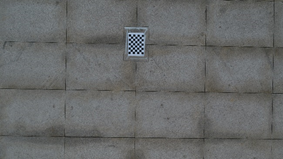
\includegraphics[width=\columnwidth]{figures/4-5a.png} 
		\subcaption{目标点1} 
		\label{fig:4-5a} 
	\end{minipage}
	\begin{minipage}[t]{0.5\linewidth} 
		\centering
		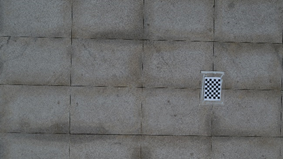
\includegraphics[width=\columnwidth]{figures/4-5b.png} 
		\subcaption{目标点2} 
		\label{fig:4-5b} 
	\end{minipage}
	\begin{minipage}[t]{0.5\linewidth} 
		\centering
		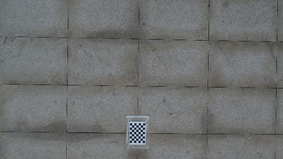
\includegraphics[width=\columnwidth]{figures/4-5c.png} 
		\subcaption{目标点3} 
		\label{fig:4-5c} 
	\end{minipage}
	\begin{minipage}[t]{0.5\linewidth} 
		\centering
		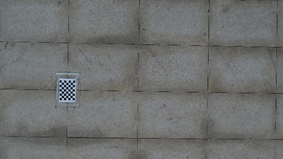
\includegraphics[width=\columnwidth]{figures/4-5d.png} 
		\subcaption{目标点4} 
		\label{fig:4-5d} 
	\end{minipage}
	\caption{目标定位测试图像}
	\label{fig:4-5}
\end{figure}

表~\ref{tab:4-2}为目标定位测试的数据和结果,测试时保持无人机在空中悬停,无人机经纬度为(30.540224°N, 114.351715°E),高度为3m,无人机经纬度和目标经纬度真实值通过高精度差分GPS设备测得,地球半径取平均半径6371.393km。

可以看到在机体坐标系下目标$(x, y)$坐标误差在10cm以内,经纬度误差在$10^{-6}$度以内,定位误差非常小,表明基于PnP算法的目标定位方案可行,并且精度可以达到10cm以内。

\clearpage
\begin{table}[htb]
	\centering
	\caption{目标定位测试结果}
	\label{tab:4-2}
	\begin{tabular}{ccccc}
		\toprule
		\multirow{2}{*}{目标序号} & \multirow{2}{*}{偏航角} & \multicolumn{3}{c}{机体坐标系下目标$(x, y)$坐标(mm)} \\ \cmidrule(l){3-5} 
		& & 真实值 & 计算值 & 误差 \\ 
		\midrule
		1 & 80° & (600, 0) & (594, -68) & \textbf{(-6, -68)} \\
		2 & 170° & (0, 900) & (21, -911) & \textbf{(21, 11)} \\
		3 & 260° & (-600, 0) & (-547, -50) & \textbf{(53, -50)} \\
		4 & 350° & (0, -900) & (2, -948) & \textbf{(2, -48)} \\		
		\toprule	
	\end{tabular}
\end{table}

\subsection{自主飞行测试}
本设计利用ROS和DJI的Onboard SDK实现无人机的自主飞行,通过将无人机的局部坐标数据发布到ROS,可以利用Rviz绘制出无人机的飞行轨迹。图~\ref{fig:4-6}显示了无人机的自主飞行轨迹,如绿线所示,可以看到实际的飞行轨迹与预设的非常接近,扫描轨迹形状与图~\ref{fig:2-18}所示完全一致,证明本设计可以很好地通过软件控制无人机自主飞行。

\begin{figure}[htb]
	\centering
	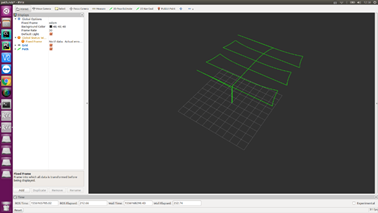
\includegraphics[width=0.6\linewidth]{figures/4-6.png}
	\caption{无人机自主飞行测试结果}
	\label{fig:4-6}
\end{figure}

\section{无人车系统测试}
\subsection{自主定位测试}
本设计采用基于里程计和激光雷达扫描匹配的自主定位方案,通过将无人车的位姿信息发布到ROS,可以利用Rviz实时显示无人车的当前位置和运动轨迹。图~\ref{fig:4-7}为无人车沿着矩形路径运动2周的轨迹,其中绿线代表无人车的运动轨迹,红色箭头代表无人车当前的位置和朝向。可以看到2次绕矩形运动的轨迹几乎重合,说明累积误差非常小,定位比较精准。

\begin{figure}[htb]
	\centering
	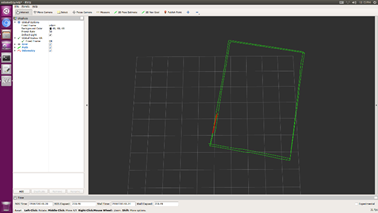
\includegraphics[width=0.6\linewidth]{figures/4-7.png}
	\caption{无人车运动轨迹}
	\label{fig:4-7}
\end{figure}

\subsection{SLAM建图测试}
SLAM建图测试的场地为实验楼走廊,图~\ref{fig:4-8}为SLAM建图结果,图中走廊的两侧墙壁非常明显,两处楼梯也正确地显示在地图中,地图没有错位现象,建图效果非常好。

\begin{figure}[htb]
	\centering
	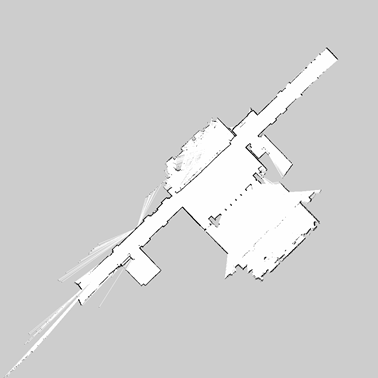
\includegraphics[width=0.6\linewidth]{figures/4-8.png}
	\caption{SLAM建图结果}
	\label{fig:4-8}
\end{figure}

\subsection{自主导航测试}
本设计采用边建图边导航的自主导航方案,图~\ref{fig:4-9}展示了自主导航的测试场地,测试时使用了一些箱子和泡沫块作为障碍物,模拟复杂环境。图~\ref{fig:4-10}展示了自主导航测试效果,图~\ref{fig:4-10a}为Rviz显示的图像,图~\ref{fig:4-10b}为对应时刻的无人车图像。图~\ref{fig:4-10a}中,较细的曲线代表无人车的路径或轨迹,其中,紫色曲线为导航算法规划的全局路径,绿色曲线为无人车的运动轨迹,绿色曲线端点处的红色箭头代表无人车当前的位置和朝向,另一处红色箭头代表目标的位置。此外,图中较粗的线条代表激光雷达检测到的障碍物,黑色线条代表地图中的障碍物边界,蓝紫色的区域代表对障碍物的膨胀,离障碍物越近颜色越浅、越危险,这是代价地图可视化的效果。

图~\ref{fig:4-10}展示的是无人车达到第一个目标点后,前往第二个目标点的过程,导航算法已经规划出了正确的全局路径,并且无人车正按着该全局路径向目标处运动。同时,建图算法已经建好了部分地图。最终无人车安全达到了所有目标点,说明无人车系统的导航算法安全、可行。

\begin{figure}[htb]
	\centering
	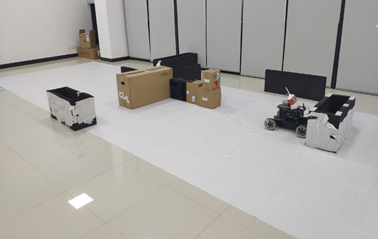
\includegraphics[width=0.6\linewidth]{figures/4-9.png}
	\caption{自主导航测试场地}
	\label{fig:4-9}
\end{figure}

\clearpage
\begin{figure}[htb]
	\centering
	\begin{minipage}[t]{\linewidth} 
		\centering
		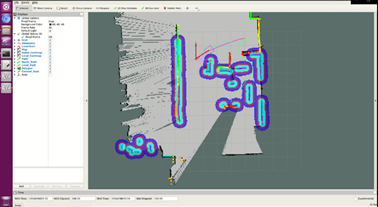
\includegraphics[width=0.6\columnwidth]{figures/4-10a.png} 
		\subcaption{Rviz显示图像} 
		\label{fig:4-10a}
	\end{minipage}
	\begin{minipage}[t]{\linewidth} 
		\centering
		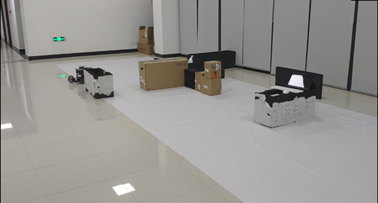
\includegraphics[width=0.6\columnwidth]{figures/4-10b.png} 
		\subcaption{无人车图像} 
		\label{fig:4-10b} 
	\end{minipage}
	\caption{自主导航测试效果}
	\label{fig:4-10}
\end{figure}

\section{系统整体测试}
图~\ref{fig:4-11}为系统整体测试的实验场地,搜索目标(基准标记)周围放置了一些泡沫块作为障碍物。图~\ref{fig:4-12}展示了测试效果,图~\ref{fig:4-12a}为无人机正在扫描搜索区域,图~\ref{fig:4-12b}为无人车正在前往目标处。测试时无人机成功检测到了目标,并比较精确地计算出了目标的GPS坐标,最终无人车成功到达了目标处。测试结果表明,本系统已经初步成型,具备了空地联合目标搜索的能力。

\begin{figure}[htb]
	\centering
	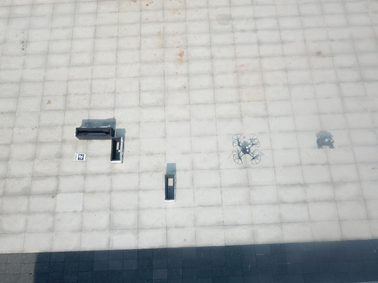
\includegraphics[width=0.4\linewidth]{figures/4-11.png}
	\caption{系统整体测试测试场地}
	\label{fig:4-11}
\end{figure}

\begin{figure}[htb]
	\centering
	\begin{minipage}[t]{\linewidth} 
		\centering
		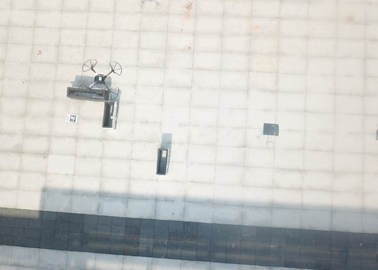
\includegraphics[width=0.5\columnwidth]{figures/4-12a.png} 
		\subcaption{无人机正在扫描搜索区域} 
		\label{fig:4-12a}
	\end{minipage}
	\begin{minipage}[t]{\linewidth} 
		\centering
		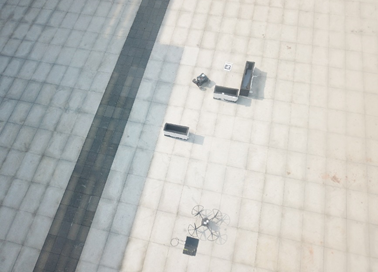
\includegraphics[width=0.5\columnwidth]{figures/4-12b.png} 
		\subcaption{无人车正在前往目标处} 
		\label{fig:4-12b} 
	\end{minipage}
	\caption{系统整体测试测试效果}
	\label{fig:4-12}
\end{figure}

\section{本章小结}
本章分别对无人机系统、无人车系统以及整体系统进行了测试与结果分析,测试结果显示,本设计的主题——基于无人机-车的空地联合目标搜索系统已经初步成型,具备了初期预想的功能。
